\documentclass[11pt]{article}

\usepackage[UTF8,fontset=fandol]{ctex}
\usepackage{lastpage}
\usepackage{extramarks}
\usepackage[usenames,dvipsnames]{color}
\usepackage{graphicx}
\usepackage{listings}
\usepackage{courier}
\usepackage{booktabs}
\usepackage{amsmath, amssymb, amsthm}
\usepackage{enumitem}
\usepackage{caption}
\usepackage{algpseudocode}
\usepackage{algorithmicx}
\usepackage[ruled]{algorithm}
\usepackage[colorlinks=true,linkcolor=blue,urlcolor=blue]{hyperref}
\usepackage{fancyhdr}

% 页边距
\topmargin=-0.45in
\evensidemargin=0in
\oddsidemargin=0in
\textwidth=6.5in
\textheight=9.0in
\headsep=0.25in

\linespread{1.05}
\setlength\parindent{0pt}

% 页眉页脚
\pagestyle{fancy}
\fancyhf{}
\lhead{\small CS 224N（2024 春季）· 默认最终项目}
\rhead{\small 第 \thepage\ 页}
\cfoot{}
\renewcommand\headrulewidth{0.4pt}

% 代码样式
\definecolor{MyDarkGreen}{rgb}{0.0,0.4,0.0}
\lstset{
  basicstyle=\footnotesize\ttfamily,
  frame=single,
  keywordstyle=\color{Blue}\bfseries,
  commentstyle=\color{MyDarkGreen},
  stringstyle=\color{Purple},
  showstringspaces=false,
  numbers=left,
  numberstyle=\tiny\color{Blue},
  breaklines=true,
  tabsize=4
}

\title{\textbf{CS 224N（2024 春季）：默认最终项目 \\ minBERT 与下游任务}}
\author{}
\date{}

\begin{document}

\maketitle
\vspace{-2em}

\begin{center}
\small\textit{说明：本项目改编自卡内基梅隆大学 CS11-711 高级自然语言处理课程的 ``minbert'' 作业，原作者为 Shuyan Zhou、Zhengbao Jiang、Ritam Dutt、Brendon Boldt、Aditya Veerubhotla 与 Graham Neubig。}
\end{center}

\tableofcontents
\newpage

%=====================================================================
\section{概述（Overview）}

默认最终项目包含两个部分。第一部分中，你将补全缺失的代码块，完成 BERT 模型的实现。随后，利用加载到你的 BERT 模型中的预训练权重，在 SST 数据集和 CFIMDB 数据集上执行情感分析。

第二部分中，你将探索 BERT 模型的扩展，从而在多个句子级任务上取得尽可能高的性能：\textbf{情感分析}、\textbf{释义检测}和\textbf{语义文本相似度}。这一部分的目标是让你设计并实验各种针对 BERT 模型的改进，以获得鲁棒且可泛化的句子嵌入，使其在不止一种场景下都有良好表现。

\textbf{关于默认项目与自定义项目的说明：}默认最终项目的本意，并不是要求比自定义最终项目更少的投入或工作量。默认项目只是省去了自己构思项目主题与评测方法的难度，让你能把等量的精力投入到给定的问题上。

\subsection{Bidirectional Encoder Representations from Transformers：BERT}

Transformers 的双向编码器表示（Bidirectional Encoder Representations from Transformers），即 ``BERT''，是一种基于 Transformer 的、能够生成上下文相关词表示的模型~\cite{devlin2018bert}。以 Transformer 为骨干、并利用双向词表示，BERT 在 2018 年发布时，为上下文词嵌入／大语言模型／基础模型领域带来了一次巨大的飞跃。

\subsection{情感分析（Sentiment Analysis）}

理解一段文本的一个基本任务是判断其\textbf{极性}，也就是文本中所表达的观点是正面的、负面的还是中性的。情感分析可用于判断个体对特定产品、政客或新闻报道的态度。

作为一个具体的情感分析数据集例子，斯坦福情感树库（Stanford Sentiment Treebank）\footnote{\url{https://nlp.stanford.edu/sentiment/treebank.html}}~\cite{socher2013recursive} 由从影评中抽取的 11{,}855 条单句组成。该数据集用斯坦福句法分析器解析\footnote{\url{https://nlp.stanford.edu/software/lex-parser.shtml}}，共包含 215{,}154 个独特短语，由 3 位人工标注者标注。每个短语的标签为\textbf{负面}、\textbf{有些负面}、\textbf{中性}、\textbf{有些正面}或\textbf{正面}。以下是从 SST 数据集中抽取的三个例子：

\begin{itemize}[leftmargin=2em]
  \item 影评：\textit{Light, silly, photographed with colour and depth, and rather a good time.}\\
        情感：4（正面）
  \item 影评：\textit{Opening with some contrived banter, cliches and some loose ends, the screenplay only comes into its own in the second half.}\\
        情感：2（中性）
  \item 影评：\textit{... a sour little movie at its core; an exploration of the emptiness that underlay the relentless gaiety of the 1920's ... The film's ending has a ``What was it all for?''}\\
        情感：0（负面）
\end{itemize}

\subsection{释义检测（Paraphrase Detection）}

释义检测是在一个大型语料库中寻找文本的\textbf{释义}的任务。释义是指``以另一种形式对文本进行重述（或复用），给出相同含义''~\cite{fernando2008semantic}。因此，释义检测旨在判断特定的词或短语是否传达相同的语义。从研究角度看，释义检测是一个有趣的任务，因为它提供了一种度量——系统能在多大程度上``理解''细粒度的语义概念。

网站 Quora\footnote{\url{https://www.quora.com/q/quoradata/First-Quora-Dataset-Release-Question-Pairs}} 经常会收到与其他问题重复的问题。为了更好地分流用户并减少不必要的工作，Quora 发布了一个数据集，标注了不同问题之间是否为彼此的释义。以下是从 Quora 数据集中抽取的两个例子：

\begin{itemize}[leftmargin=2em]
  \item 问题对：(1) \textit{"What is the step by step guide to invest in share market in india?"}，(2) \textit{"What is the step by step guide to invest in share market?"}\\
        是否为释义：否
  \item 问题对：(1) \textit{"I am a Capricorn Sun Cap moon and cap rising...what does that say about me?"}，(2) \textit{"I'm a triple Capricorn (Sun, Moon and ascendant in Capricorn) What does this say about me?"}\\
        是否为释义：是
\end{itemize}

\subsection{语义文本相似度（Semantic Textual Similarity, STS）}

语义文本相似度（STS）任务旨在刻画``有些文本比其他文本更相似''这一概念；STS 试图度量\textbf{语义等价的程度}~\cite{agirre2013sem}。STS 与释义检测的区别在于，它不是一个非是即否的判断，而是允许存在相似度的\textbf{程度}。例如，在从 0（毫不相关）到 5（含义相同）的标度上，以下句子的相似度评分如下\footnote{这些句子与标签来自 \url{https://aclanthology.org/S13-1004.pdf}~\cite{agirre2013sem}。}：

\begin{itemize}[leftmargin=2em]
  \item \textbf{(5)} 两个句子完全等价，含义完全相同：\\
        \textit{The bird is bathing in the sink.}\\
        \textit{Birdie is washing itself in the water basin.}
  \item \textbf{(4)} 两个句子基本等价，仅有一些不重要的细节不同：\\
        \textit{In May 2010, the troops attempted to invade Kabul.}\\
        \textit{The US army invaded Kabul on May 7th last year, 2010.}
  \item \textbf{(3)} 两个句子大致等价，但某些重要信息不同：\\
        \textit{John said he is considered a witness but not a suspect.}\\
        \textit{``He is not a suspect anymore.''}
  \item \textbf{(2)} 两个句子不等价，但共享一些细节：\\
        \textit{They flew out of the nest in groups.}\\
        \textit{They flew into the nest together.}
  \item \textbf{(1)} 两个句子不等价，但属于同一主题：\\
        \textit{The woman is playing the violin.}\\
        \textit{The young lady enjoys listening to the guitar.}
  \item \textbf{(0)} 两个句子分属不同主题：\\
        \textit{John went horseback riding at dawn with a whole group of friends.}\\
        \textit{Sunrise at dawn is a magnificent view to take in if you wake up early enough for it.}
\end{itemize}

\subsection{本项目（This Project）}

本项目的目标是让你实现原始 BERT 模型的一些关键部分，并探索各种扩展以改进你的基线模型。第一部分聚焦于实现原始 BERT 模型的\textbf{多头自注意力层}和\textbf{Transformer 层}。随后，你将利用完成的 BERT 模型，在斯坦福情感树库数据集以及另一个影评数据集上执行情感分析。在本项目的后半部分，你将扩展你的 BERT 模型，以提升它在各类下游任务上的表现，并把模型的预测提交到全班范围的竞赛中。在第~5 节中，我们描述了若干常用于在 BERT 模型中构建更鲁棒、语义更丰富的句子嵌入的技术——其中大多数来自近期研究论文。我们提供这些建议以帮助你入门。

尽管并不要求你实现完全原创的东西，但最优秀的项目会追求某种形式的原创性，实际上甚至可能在未来成为研究论文。原创性并不一定意味着全新的方法。对现有模型做出\textbf{小而动机充分}的改动是有价值的，尤其是当改动之后还辅以严谨而有逻辑的分析时。如果你能以定量和定性的方式证明，你对最先进模型所做的小而有原创性的改动确实带来了提升（更进一步，还能解释它解决了什么具体问题、是如何解决的），那就说明你做得极其出色。

与自定义最终项目一样，默认最终项目的第二部分是开放式的。如何探索各种可能性完全由你决定。我们期望你运用迄今为止在课堂上积累的判断力和直觉，构建出性能最高的模型。有关评分标准的更多信息，请参见第~7 节。

\textbf{请注意，本文档只描述默认最终项目的编码部分。}有关报告（write-up）的更多细节，请参见课程网站以及《CS224N：项目报告说明》讲义。

%=====================================================================
\section{开始（Getting Started）}

要完成本项目，你需要一台带 GPU 的机器来高效地训练模型。为此，与作业 4 和作业 5 类似，你可以使用 Google Cloud。

我们建议你在本地机器（或斯坦福的机器，如 \texttt{rice}）上用不带 GPU 的 PyTorch 开发代码，等调试完代码、准备训练时再迁移到 Google Cloud 虚拟机上。我们建议你使用\textbf{私有} GitHub 仓库来管理代码库，并在两台机器之间以及队友之间同步文件。第一次走完本``开始''章节的流程时，请在你的本地机器上进行。之后你会在 Google Cloud 虚拟机上重复这一过程。

进入合适的机器后，用以下命令克隆项目的 GitHub 仓库：

\begin{lstlisting}[numbers=none]
https://github.com/amahankali10/CS224N-Spring2024-DFP-Student-Handout
\end{lstlisting}

该仓库包含起始代码，以及我们将使用的一个极简 BERT 模型实现（minBERT）。我们鼓励你通过 \texttt{git clone} 来克隆我们的仓库，而不是简单下载，这样你就能方便地把我们所做的任何 bug 修复整合进代码中。实际上，你应该定期检查是否有需要下载的新修复。为此，在仓库目录内运行 \texttt{git pull} 命令即可。

如果你用 GitHub 管理代码，\textbf{必须保持仓库为私有}。

\subsection{代码概览（Code overview）}

仓库 \texttt{minbert-default-final-project/} 包含以下文件：

\begin{itemize}[leftmargin=1.5em]
  \item \textbf{应保持不编辑的文件：}
    \begin{itemize}
      \item \texttt{base\_bert.py}：一个可以加载预训练权重的基础 BERT 实现。
      \item \texttt{config.py}：用于运行时配置的类。
      \item \texttt{optimizer\_test.npy}：一个包含 \texttt{optimizer\_test.py} 所需权重的 NumPy 文件。
      \item \texttt{optimizer\_test.py}：针对你完成的 Adam 优化器的测试。
      \item \texttt{sanity\_check.data}：供 \texttt{sanity\_check.py} 使用的数据文件。
      \item \texttt{sanity\_check.py}：针对你完成的 \texttt{bert.py} 文件的测试。
      \item \texttt{tokenizer.py}：实现用于文本预处理的 \texttt{BertTokenizer}。
      \item \texttt{utils.py}：工具函数与类。
    \end{itemize}
  \item \textbf{第一部分需补全缺失代码块的文件：}
    \begin{itemize}
      \item \texttt{bert.py}：你对 BERT 模型的实现。
      \item \texttt{classifier.py}：用于运行情感分析的分类流水线。
      \item \texttt{optimizer.py}：你对 Adam 优化器的实现。
    \end{itemize}
  \item \textbf{第二部分的核心文件：}
    \begin{itemize}
      \item \texttt{multitask\_classifier.py}：一个分类流水线，你将在此训练你的 minBERT 实现，使其同时执行情感分析、释义检测和语义文本相似度任务。该文件中有缺失的代码块。
      \item \texttt{datasets.py}：加载三个下游任务数据的函数与类。你可以按需编辑此文件。
      \item \texttt{evaluation.py}：在三个下游任务上评测输入模型的函数。你大概率无需编辑此文件。
    \end{itemize}
\end{itemize}

此外，还有两个目录：

\begin{itemize}[leftmargin=1.5em]
  \item \texttt{data/}：该目录包含 sst 和 cfimdb 数据集的训练、开发、测试划分，以 \texttt{.csv} 文件形式存放，将在本项目的上半部分使用。该目录还包含后半部分将用到的后续数据集的训练、开发、测试划分。注意，我们\textbf{不提供测试集的标签}。
  \item \texttt{predictions/}：该目录将存放你的模型在每个给定数据集上的输出预测。
\end{itemize}

\subsection{环境配置（Setup）}

进入合适的机器并克隆项目仓库后，就可以运行配置命令了。

\begin{itemize}[leftmargin=1.5em]
  \item 确保已安装 Anaconda 或 Miniconda。
  \item 进入 \texttt{minbert-default-final-project} 目录，运行 \texttt{source setup.sh}
    \begin{itemize}
      \item 这会创建一个名为 \texttt{cs224n\_dfp} 的 conda 环境。
      \item 除了默认安装的包外，你可能还需要安装以下包：\texttt{zipp-3.11.0}、\texttt{idna-3.4} 和 \texttt{chardet-4.0.0}。
      \item 在本项目的第一部分，你\textbf{只允许使用} \texttt{setup.sh} 安装的库。不允许使用其他任何外部库（例如 \texttt{transformers}）。
    \end{itemize}
  \item 运行 \texttt{conda activate cs224n\_dfp}
    \begin{itemize}
      \item 这会激活 \texttt{cs224n\_dfp} 环境。
      \item 记得每次写代码时都先执行这一步。
    \end{itemize}
  \item （可选）如果你想使用 PyCharm，请选择 \texttt{cs224n\_dfp} 环境。以下以 Mac OS X 为例：
    \begin{itemize}
      \item 在 PyCharm 中打开 \texttt{minbert-default-final-project} 目录。
      \item 前往 \texttt{PyCharm > Preferences > Project > Project interpreter}。
      \item 点击右上角的齿轮，然后点击 \texttt{Add}。
      \item 选择 \texttt{Conda environment > Existing environment}，点击右侧的 \texttt{...}。
      \item 选择 \texttt{/Users/YOUR\_USERNAME/miniconda3/envs/cs224n\_dfp/bin/python}。
      \item 点击 \texttt{OK} 然后点击 \texttt{Apply}。
    \end{itemize}
\end{itemize}

%=====================================================================
\section{实现 minBERT（Implementing minBERT）}

我们已经为你提供了实现 minBERT 所需的若干构建模块。本节中，我们将描述基线 BERT 模型，以及你必须实现的部分。

\subsection{BERT 的细节（Details of BERT）}

这里我们梳理 BERT 的架构，并简要提及 BERT 原始训练过程的细节。

\subsubsection{分词（\texttt{tokenizer.py}）}

BERT 模型在进一步处理之前，先把句子输入转换成 token。具体来说，BERT 使用一种 WordPiece 分词器，把句子切分成词片（word pieces）。BERT 预定义了 3 万个不同的词片。这些词片随后被转换成 id，供 BERT 模型的其余部分使用。举例来说，以下单词会被转换成以下词片：

\begin{center}
\begin{tabular}{ll}
  \toprule
  \textbf{单词} & \textbf{词片} \\
  \midrule
  snow        & [snow] \\
  snowing     & [snow, \#\#ing] \\
  fight       & [fight] \\
  fighting    & [fight,\#\#ing] \\
  snowboard   & [snow,\#\#board] \\
  \bottomrule
\end{tabular}
\end{center}

除了把每个句子切分成其组成词片的 token 之外，此前从未见过的词片（即不属于原始 3 万词片的词片）会被设为 \texttt{[UNK]} token。

为确保所有输入句子长度一致，每个输入句子会用 \texttt{[PAD]} token 填充到给定的 \texttt{max\_length}（512）。最后，对于许多下游任务，BERT 的第一个 token 的隐藏状态通常被用作整个句子的嵌入。为此，\texttt{[CLS]} token 会被添加到每个输入句子 token 表示的最前面。在本作业的第一部分，你将使用这个 token 的隐藏状态。

最后，BERT 使用 \texttt{[SEP]} token 在两个输入句子之间人为地引入分隔。这个分隔 token 对 BERT 的``下一句预测''预训练任务至关重要，但对我们情感分析任务来说基本无关紧要。

\subsubsection{嵌入层（\texttt{bert.BertModel.embed}）}

在分词并把每个 token 转换成 id 之后，BERT 模型在每个 token 上使用一个可训练的嵌入层。BERT 后续部分使用的输入嵌入是\textbf{词元嵌入}、\textbf{分段嵌入}和\textbf{位置嵌入}之和（图~\ref{fig:embedding}）。BERT 基础版本中每个嵌入层的维度都是 768。

可学习的词元嵌入把各个输入 id 映射成向量表示以供后续使用。更具体地说，给定一些输入的词片索引\footnote{词元索引是一个整数，它告诉你嵌入矩阵的哪一行（或哪一列）包含该词的嵌入。} $w_1, \dots, w_k \in \mathbb{N}$，嵌入层执行一次嵌入查表，把索引转换成词元嵌入 $v_1, \dots, v_k \in \mathbb{R}^D$。

可学习的分段嵌入用于区分句子类型。在本项目中，我们只考虑单个句子，不做下一句预测任务，因此在我们提供的代码库中，分段嵌入是用占位符实现的。

\begin{figure}[h]
  \centering
  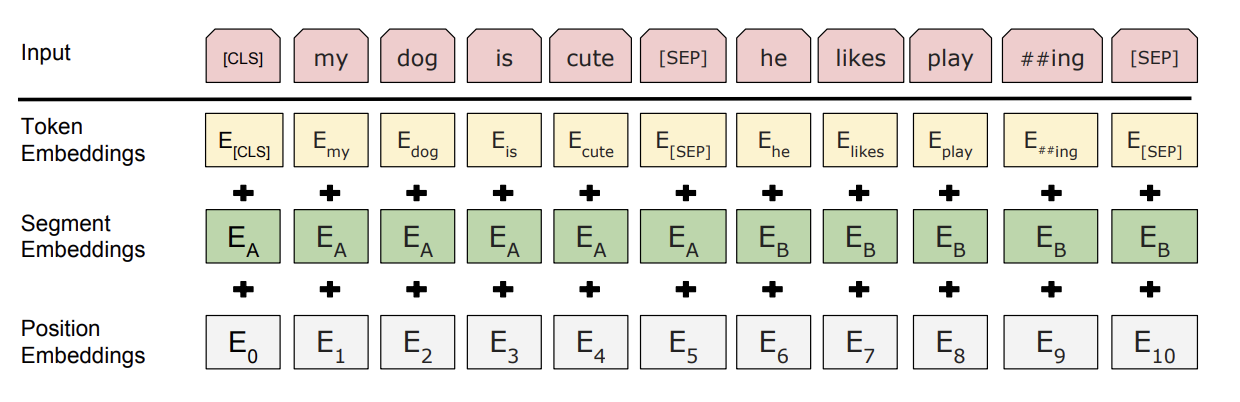
\includegraphics[width=0.85\textwidth]{fig1_embedding.png}
  \caption{BERT 嵌入层。模型后续使用的输入嵌入是词元嵌入、分段嵌入与位置嵌入之和。图取自文献~\cite{devlin2018bert} 的 Figure 2。}
  \label{fig:embedding}
\end{figure}

最后，位置嵌入用于编码输入中不同词的位置。与词元嵌入类似，位置嵌入也是参数化嵌入，为给定 BERT 输入的 512 个位置中的每一个学习一个。

\begin{figure}[h]
  \centering
  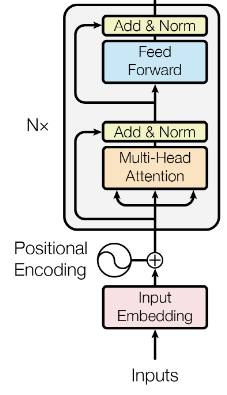
\includegraphics[width=0.42\textwidth]{fig2_encoder.png}
  \caption{BERT 中使用的 Transformer 编码器层。图取自文献~\cite{vaswani2017attention} 的 Figure 1 左半部分。}
  \label{fig:encoder}
\end{figure}

\subsubsection{BERT Transformer 层（\texttt{bert.BertLayer}）}

如原始 BERT 论文~\cite{devlin2018bert} 所述，基础版 BERT 使用了 12 个编码器 Transformer 层。这些层最初是在《Attention is All You Need》~\cite{vaswani2017attention} 一文中定义的。如图~\ref{fig:encoder} 所示，BERT Transformer 的 Transformer 层由\textbf{多头注意力}、一个带残差连接的\textbf{加法与归一化层}、一个\textbf{前馈层}，以及最后一个带残差连接的加法与归一化层组成。我们在这里简要介绍其中的每一层。我们建议你阅读上述两篇论文的第 3 节以获取更多细节。

\textbf{多头注意力（\texttt{bert.BertSelfAttention.attention}）} 多头注意力层~\cite{vaswani2017attention} 是 Transformer 架构的核心，它基于序列中其他元素来变换每个元素的隐藏状态（全连接层则是对每个元素分别作用）。我们记为 $\mathrm{MH}(\cdot)$ 的多头层由 $n$ 个不同的点积注意力机制组成。在高层面上，注意力把一个序列元素表示为所有序列元素隐藏状态的加权和。在多头注意力中，求和里的权重使用变换后隐藏状态之间的点积相似度。具体来说，第 $i$ 个注意力机制``头''为：

\begin{equation}
\mathrm{Attention}_i(h_j) = \sum_t \mathrm{softmax}\left(\frac{W_i^q h_j \cdot W_i^k h_t}{\sqrt{d/n}}\right) W_i^v h_t
\end{equation}

其中 $h_j$（为简化，在后续公式中我们将省略下标 $j$）是某个特定序列元素的 $d$ 维隐藏向量，$t$ 遍历每一个序列元素。在 BERT 中，$W_i^q$、$W_i^k$ 和 $W_i^v$ 是大小为 $d/n \times d$ 的矩阵，因此每个``头''都会投影到一个大小为 $d/n$ 的不同子空间，关注不同的信息。

最后，$n$ 个注意力头（每个大小为 $d/n$）的输出被拼接在一起（我们用 $[\cdot, \dots, \cdot]$ 表示），并用 $W^o$（一个 $d \times d$ 矩阵）进行线性变换\footnote{文献~\cite{vaswani2017attention} 提供了更详细的动机与讨论。}：

\begin{equation}
\mathrm{MH}(h) = W^o [\mathrm{Attention}_1(h), \dots, \mathrm{Attention}_n(h)]
\end{equation}

我们进一步定义 BERT 层的另一个组成部分——自注意力层，记为 $\mathrm{SA}(\cdot)$：

\begin{equation}
h' = \mathrm{LN}(h + \mathrm{MH}(h))
\end{equation}

\begin{equation}
\mathrm{SA}(h) = \mathrm{FFN}(h')
\end{equation}

$\mathrm{LN}(\cdot)$ 是层归一化~\cite{ba2016layer}。$\mathrm{FFN}$ 是一个标准的前馈网络：

\begin{equation}
\mathrm{FFN}(h) = W_2 f(W_1 h + b_1) + b_2
\end{equation}

其中 $f(\cdot)$ 是一个非线性函数，在 BERT 中为 GeLU~\cite{hendrycks2016gaussian}。矩阵 $W_1$ 的大小为 $d_{ff} \times d$，$W_2$ 的大小为 $d \times d_{ff}$。综合起来，一个 BERT 层，记为 $\mathrm{BL}(\cdot)$，就是对自注意力层的输出施加带残差连接的层归一化：

\begin{equation}
\mathrm{BL}(h) = \mathrm{LN}(h' + \mathrm{SA}(h))
\end{equation}

\textbf{Dropout} 最后我们指出，BERT 对每个子层的输出应用 dropout，之后再将其与子层输入相加并归一化。BERT 还对嵌入之和与位置编码之和应用 dropout。BERT 使用的设置为 $p_{drop} = 0.1$。

\subsubsection{BERT 输出（\texttt{bert.BertModel.forward}）}

如本节所述，BERT 由以下部分组成：

\begin{enumerate}
  \item 一个嵌入层，由一个词嵌入器和一个位置嵌入器组成。
  \item BERT 编码器层，即一堆 \texttt{config.num\_hidden\_layers}（在我们的例子中为 12）个 \texttt{BertLayer}。
\end{enumerate}

模型输出包括：

\begin{enumerate}
  \item \texttt{last\_hidden\_state}：来自最后一个 \texttt{BertLayer} 的句子中每个词片的上下文化嵌入（即 BERT 编码器的输出）。
  \item \texttt{pooler\_output}：\texttt{[CLS]} token 的嵌入。
\end{enumerate}

\subsubsection{训练 BERT（Training BERT）}

原始版本的 BERT 是在维基百科文章上，用两个无监督任务训练出来的。

\begin{figure}[h]
  \centering
  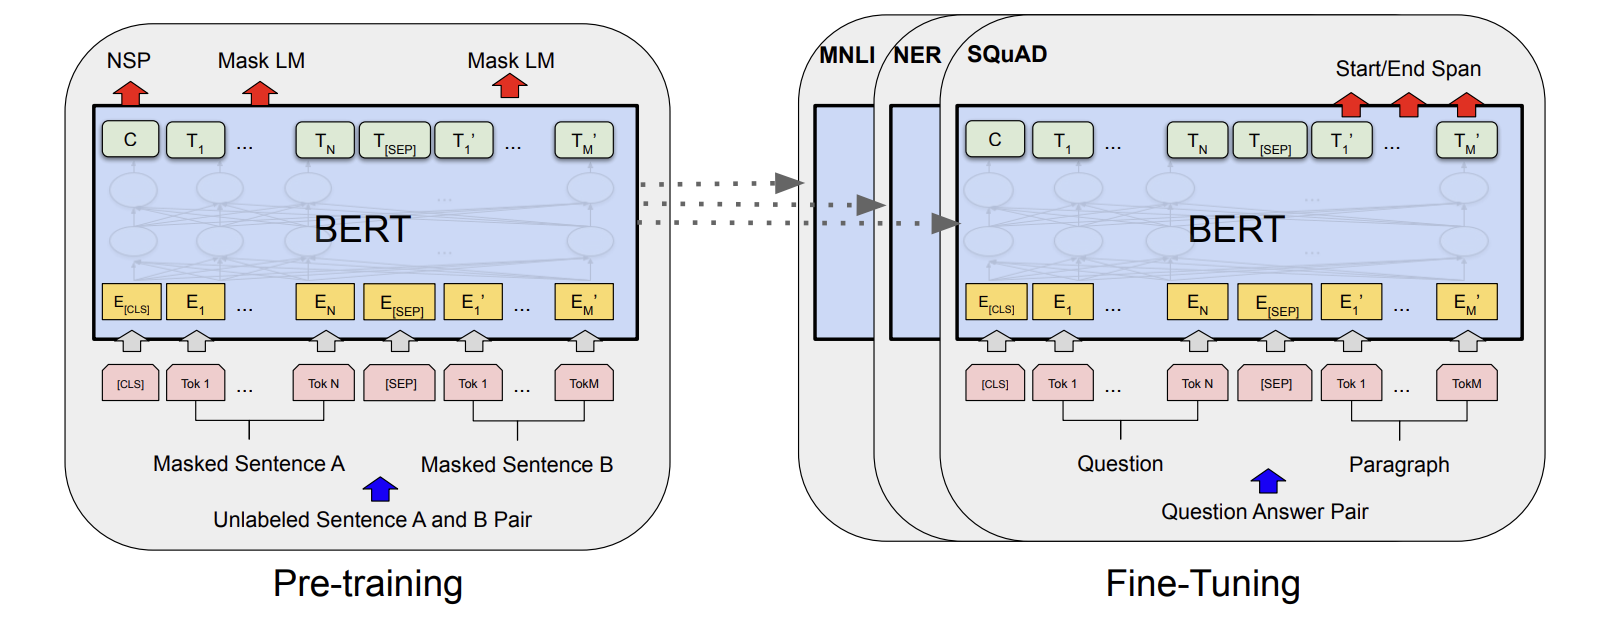
\includegraphics[width=0.9\textwidth]{fig3_pretraining.png}
  \caption{原始 BERT 模型在两个无监督任务上训练：掩码 token 预测和下一句预测。图取自文献~\cite{devlin2018bert} 的 Figure 1。}
  \label{fig:pretraining}
\end{figure}

\textbf{掩码语言建模（Masked Language Modeling）} 为了让 BERT 学会提取深度的双向表示，训练过程会掩盖一定比例（原始论文中为 15\%）的词片 token，并尝试预测它们。具体来说，与被掩码 token 对应的最终隐藏向量会被送入一个覆盖整个词表的输出 softmax 层，随后被预测出来。

为了防止初始预训练与后续微调之间出现不匹配，``被掩码''的 token 在训练期间并非总是被替换为 \texttt{[MASK]} token。相反，训练数据生成器会随机选择 15\% 的 token 位置用于预测；然后，被选中的 token 中有 80\% 被替换为 \texttt{[MASK]}，10\% 被替换为随机 token，另外 10\% 保持不变。

\textbf{下一句预测（Next Sentence Prediction）} 为了让 BERT 理解两个句子之间的关系，BERT 还会在下一句预测任务上进一步微调。具体来说，BERT 模型有 50\% 的时间看到一个句子及其下一个句子；另外 50\% 的时间则看到一个随机的第二个句子。BERT 模型需要预测第二个输入句子是否真的是下一个句子。

\subsection{待实现代码：多头自注意力与 Transformer 层}

我们已经为你提供了 BERT 基线模型的大部分代码。在梳理完 BERT Transformer 模型的基本结构后，我们现在描述需要实现的部分：

\subsubsection{BERT 多头自注意力：\texttt{bert.BertSelfAttention.attention}}

你必须实现 Transformer 的多头注意力层。该层把一个查询和一组键值对映射到一个输出。输出计算为值的加权和，其中每个值的权重由一个以查询和键为输入的函数计算得出。

\subsubsection{BERT Transformer 层：\texttt{bert.BertLayer} 与 \texttt{bert.BertModel}}

实现 BERT 多头自注意力层之后，你还必须实现若干函数，以实现完整的 BERT Transformer 层。这些代码块位于 \texttt{bert.BertLayer.add\_norm}、\texttt{bert.BertLayer.forward} 和 \texttt{bert.BertModel.embed}。

完成这些步骤后，你可以运行一个 sanity check 来验证你实现的正确性：

\begin{lstlisting}[numbers=none]
python sanity_check.py
\end{lstlisting}

该 sanity check 会加载我们用参考实现计算出的两个嵌入，并检查你的实现输出是否与我们的匹配。

%=====================================================================
\section{用 BERT 做情感分析（Sentiment Analysis with the BERT）}

实现一个可用的 minBERT 模型后，你现在将利用预训练模型权重，以及你所实现的 BERT 模型的输出嵌入，在两个数据集上执行情感分析。除了加载这些预训练模型权重外，你还要（像作业 5 那样）在每个数据集上微调这些嵌入，以获得更好的结果。你可以在 \texttt{data} 子文件夹中找到这两个数据集。

\subsection{数据集（Datasets）}

\subsubsection{斯坦福情感树库（Stanford Sentiment Treebank, SST）数据集}

斯坦福情感树库\footnote{\url{https://nlp.stanford.edu/sentiment/treebank.html}}~\cite{socher2013recursive} 由从影评中抽取的 11{,}855 条单句组成。该数据集用斯坦福句法分析器解析\footnote{\url{https://nlp.stanford.edu/software/lex-parser.shtml}}，从那些解析树中得到了总计 215{,}154 个独特短语，由 3 位人工标注者标注。每个短语的标签为\textbf{负面}、\textbf{有些负面}、\textbf{中性}、\textbf{有些正面}或\textbf{正面}。你将利用 BERT 嵌入来预测这些情感分类标签。

对于 SST 数据集，我们有如下划分：
\begin{itemize}[leftmargin=1.5em]
  \item train（8{,}544 个样本）
  \item dev（1{,}101 个样本）
  \item test（2{,}210 个样本）
\end{itemize}

\subsubsection{CFIMDB 数据集}

CFIMDB 数据集由 2{,}434 条情感极性极强的影评组成。每条影评有一个二分类标签：\textbf{负面}或\textbf{正面}。你将利用 BERT 嵌入来预测这些情感分类。

对于 CFIMDB 数据集，我们有如下划分：
\begin{itemize}[leftmargin=1.5em]
  \item train（1{,}701 个样本）
  \item dev（245 个样本）
  \item test（488 个样本）
\end{itemize}

\subsection{待实现代码：基于 BERT 嵌入的情感分类}

在 \texttt{classifier.py} 文件中，你会找到一个流水线，它为两个数据集执行以下操作：
\begin{enumerate}
  \item 调用 BERT 模型对句子进行编码，得到它们的上下文化表示；
  \item 在句子分类样本上训练并评测你的 BERT 模型；
  \item 保存你的预测。
\end{enumerate}

在该文件中，你要实现 \texttt{BertSentimentClassifer}。这个类用 BERT 对句子进行编码，并得到每个句子的池化表示\footnote{参见 \texttt{bert.py} 中的 \texttt{forward} 函数，了解如何获取这一表示。}。然后，它对池化输出应用 dropout，再用一个线性层将其投影，从而对句子进行分类。已经实现的部分包括：模型根据我们是在使用预训练权重还是在微调，来冻结或训练参数的能力。

\subsection{Adam 优化器（Adam Optimizer）}

除了实现 \texttt{BertSentimentClassifer} 之外，你还要基于《Decoupled Weight Decay Regularization》~\cite{loshchilov2017decoupled} 和《Adam: A Method for Stochastic Optimization》~\cite{kingma2014adam} 实现 Adam 优化器的 \texttt{step()} 函数。

\subsubsection{Adam 优化器概述}

Adam 优化器是一种高效随机优化的方法，只需要一阶梯度。该方法通过估计梯度的一阶矩和二阶矩，为不同参数计算自适应学习率。具体来说，在每个时间步，算法更新梯度 $m_t$ 和平方梯度 $v_t$ 的指数移动平均，其中超参数 $\beta_1, \beta_2 \in [0, 1)$ 控制这些平均值的指数衰减速率。由于这些移动平均在初始时间步被初始化为 0，它们会偏向于零。因此，该算法的一个关键方面是在每个时间步执行\textbf{偏差校正}，得到 $\hat{m}_t$ 和 $\hat{v}_t$。下面给出完整算法：

\begin{algorithm}[h]
\caption{Adam 算法。$g_t^2$ 表示逐元素平方 $g_t \odot g_t$。所有对向量的操作都是逐元素的。我们用 $\beta_1^t$ 和 $\beta_2^t$ 表示 $\beta_1$ 和 $\beta_2$ 的 $t$ 次方。}
\begin{algorithmic}[1]
\Require $\alpha$：步长
\Require $\beta_1, \beta_2 \in [0, 1)$：矩估计的指数衰减率
\Require $f(\theta)$：以 $\theta$ 为参数的随机目标函数
\Require $\theta_0$：初始参数向量
\State $m_0 \leftarrow 0$ \Comment{初始化一阶矩向量}
\State $v_0 \leftarrow 0$ \Comment{初始化二阶矩向量}
\State $t \leftarrow 0$ \Comment{初始化时间步}
\While{$\theta_t$ 未收敛}
  \State $t \leftarrow t + 1$
  \State $g_t \leftarrow \nabla f_t(\theta_{t-1})$ \Comment{在时间步 $t$ 获取随机目标函数的梯度}
  \State $m_t \leftarrow \beta_1 \cdot m_{t-1} + (1 - \beta_1) \cdot g_t$ \Comment{更新有偏一阶矩估计}
  \State $v_t \leftarrow \beta_2 \cdot v_{t-1} + (1 - \beta_2) \cdot g_t^2$ \Comment{更新有偏二阶原始矩估计}
  \State $\hat{m}_t \leftarrow m_t / (1 - \beta_1^t)$ \Comment{计算偏差校正后的一阶矩估计}
  \State $\hat{v}_t \leftarrow v_t / (1 - \beta_2^t)$ \Comment{计算偏差校正后的二阶原始矩估计}
  \State $\theta_t \leftarrow \theta_{t-1} - \alpha \cdot \hat{m}_t / (\sqrt{\hat{v}_t} + \epsilon)$
\EndWhile
\State \textbf{return} $\theta_t$ \Comment{返回结果参数}
\end{algorithmic}
\end{algorithm}

注意，以牺牲清晰度为代价，上述算法存在一个更高效的版本，其中循环里的最后三行被替换为以下两行：$\alpha_t \leftarrow \alpha \cdot \sqrt{1 - \beta_2^t} / (1 - \beta_1^t)$ 以及 $\theta_t \leftarrow \theta_{t-1} - \alpha_t \cdot m_t / (\sqrt{v_t} + \epsilon)$。

\subsubsection{待实现代码：\texttt{optimizer.step}}

你应该实现 Adam 优化器的 \texttt{step()} 函数。我们的参考实现使用了文献~\cite{kingma2014adam} 第 2 节``Algorithm''中介绍的``高效''偏差校正计算方法，上述伪代码中也有提及。最后，你应该纳入权重衰减（通过在损失函数中加入 $\frac{\lambda}{2}\theta_t^2$，等价于在每个梯度下降步骤结束时从参数中减去 $\alpha\lambda\theta_t$，其中 $\lambda$ 是权重衰减正则化参数），作为对参数的最终更新。你可以运行以下命令来测试你的实现：

\begin{lstlisting}[numbers=none]
python3 optimizer_test.py
\end{lstlisting}

\subsection{训练 minBERT 做情感分类}

完成第一部分的实现后，你将用预训练和微调后的嵌入，在 SST 和 CFIMDB 数据集上试验你完成的模型。你可以用以下命令运行训练：

\begin{lstlisting}[numbers=none]
python3 classifier.py --fine-tune-mode {full-model,last-linear-layer} --lr {1e-3,1e-5}
\end{lstlisting}

每个数据集的训练不应超过 5 到 15 分钟（取决于你的 GPU）。运行 \texttt{last-linear-layer} 时使用学习率 $10^{-3}$，运行 \texttt{full-model} 时使用学习率 $10^{-5}$。之后，检查你的 \texttt{predictions} 目录中是否生成了以下 8 个文件：

\begin{lstlisting}[numbers=none]
{full-model,last-linear-layer}-sst-dev-out.csv
{full-model,last-linear-layer}-sst-test-out.csv
{full-model,last-linear-layer}-cfimdb-dev-out.csv
{full-model,last-linear-layer}-cfimdb-test-out.csv
\end{lstlisting}

作为基线，你的实现应该得到与以下相近的结果（括号内为 10 个随机种子上的平均参考准确率及其标准差）：

\begin{itemize}[leftmargin=1.5em]
  \item 对 SST 微调最后一个线性层：Dev Accuracy：0.390 (0.007)
  \item 对 CFIMDB 微调最后一个线性层：Dev Accuracy：0.780 (0.002)
  \item 对 SST 微调完整模型：Dev Accuracy：0.515 (0.004)
  \item 对 CFIMDB 微调完整模型：Dev Accuracy：0.966 (0.007)
\end{itemize}

你\textbf{只能}使用我们提供的训练集和开发集来训练、调优和评测你的模型。如果你把这些数据集的官方测试数据用于训练、调优或评测你的模型，或者以任何方式手动修改你的 CSV 答案，就构成\textbf{荣誉准则违规}。对于这一部分，评分时我们主要考察你的代码/实现（以及你在测试集上的准确率）。

\subsection{minBERT 的提交说明}

你将在 Gradescope 上提交本项目的 minBERT 部分：

\begin{enumerate}
  \item 验证以下文件在你的作业目录中的指定路径下存在：
    \begin{itemize}
      \item \texttt{bert.py}
      \item \texttt{classifier.py}
      \item \texttt{optimizer.py}
      \item \texttt{predictions/\{full-model,last-linear-layer\}-sst-dev-out.csv}
      \item \texttt{predictions/\{full-model,last-linear-layer\}-sst-test-out.csv}
      \item \texttt{predictions/\{full-model,last-linear-layer\}-cfimdb-dev-out.csv}
      \item \texttt{predictions/\{full-model,last-linear-layer\}-cfimdb-test-out.csv}
    \end{itemize}
  \item 运行 \texttt{prepare\_submit.py}，生成你的 \texttt{cs224n\_default\_final\_project\_submission.zip} 文件。
  \item 将你的 \texttt{cs224n\_default\_final\_project\_submission.zip} 文件上传到 GradeScope 上相应的作业。
\end{enumerate}

在高层面，SST 和 CFIMDB 开发/测试数据集的提交文件应大致如下所示：

\begin{lstlisting}[numbers=none]
id, Predicted_Sentiment
001fefa37a13cdd53fd82f617, 4
00415cf9abb539fbb7989beba, 2
00a4cc38bd041e9a4c4e545ff, 1
...
fffcaebf1e674a54ecb3c39df, 3
\end{lstlisting}

%=====================================================================
\section{针对额外下游任务的扩展与改进}

虽然我们在项目的前半部分聚焦于实现 BERT 的关键部分，但在项目的其余部分（也是构成你最终项目大部分分数的部分），你将可以自由地探索其他数据集，以更好地微调或以其他方式调整你的 BERT 嵌入，使其能够\textbf{同时}执行以下三个任务：情感分析、释义检测和语义文本相似度。后半部分的目标是探索如何构建能在大量不同任务上都表现良好的鲁棒嵌入！

在本节中，我们将使用 SST 数据集做情感分析、Quora 数据集做释义检测、SemEval 数据集做语义文本相似度。你可以在 \texttt{data} 文件夹中找到每个数据集的训练、开发、测试集。你\textbf{只能}使用我们的训练集和开发集来训练、调优和评测你的模型。如果你把这些数据集的官方测试数据用于训练、调优或评测你的模型，或者以任何方式手动修改你的 CSV 答案，就构成\textbf{荣誉准则违规}。

除了第一部分提供给你的、从预训练 BERT 权重中提取的嵌入之外，你还可以使用其他既有的 NLP 工具，如词性标注器、依存句法分析器、WordNet、共指消解模块等，只要它们不是建立在你的训练嵌入之上的。你对外部资源的使用被限制在合理范围内。例如，你\textbf{不可以}使用 \texttt{transformers} 库中的预训练嵌入。

\subsection{数据集概览（Dataset Overview）}

\subsubsection{Quora 数据集}

如第 1 节所述，Quora 数据集由 404{,}298 个问题对组成，并带有标签，表明特定实例是否为彼此的释义。我们为你提供了如下划分：

\begin{itemize}[leftmargin=1.5em]
  \item train（283{,}010 个样本）
  \item dev（40{,}429 个样本）
  \item test（80{,}859 个样本）
\end{itemize}

由于该数据集是二分类标签，我们用准确率来评测你的表现。

\subsubsection{SemEval STS 基准数据集}

如第 1 节所述，SemEval STS 基准数据集由 8{,}628 个不同的句子对组成，相似度在从 0（不相关）到 5（含义等价）的标度上各不相同。

对于 STS 数据集，我们有如下划分：

\begin{itemize}[leftmargin=1.5em]
  \item train（6{,}040 个样本）
  \item dev（863 个样本）
  \item test（1{,}725 个样本）
\end{itemize}

评测该数据集时，与原始 SemEval 论文~\cite{agirre2013sem} 一样，我们将使用真实相似度值与预测相似度值之间的 Pearson 相关系数。

\subsection{代码概览（Code Overview）}

我们为你提供了一组类与函数（其中一些包含缺失的代码块），以帮助你训练和评测本项目的第二部分。对于这一部分，我们不会对你的代码评分，因此你可以自由地重新组织、创建新的类和函数，或以其他方式改造你的旧代码。这里我们简要概述所提供的代码：

\begin{itemize}[leftmargin=1.5em]
  \item \texttt{multitask\_classifier.MultitaskBERT}：一个导入预训练 BERT 模型权重、并预测情感、释义和语义文本相似度的类。
  \item \texttt{multitask\_classifier.MultitaskBERT.forward}：调用你之前实现的 BERT 模型输出句子嵌入。你可以选择试验特定词片的上下文词嵌入，或像 \texttt{classifier.py} 那样只提取 \texttt{pooler\_output}。
  \item \texttt{multitask\_classifier.MultitaskBERT.predict\_sentiment}：基于 BERT 嵌入预测句子的情感。作为基线，你应该像 \texttt{classifier.py} 那样，调用上面的新 \texttt{forward()} 方法，再接一个 dropout 和线性层。
  \item \texttt{multitask\_classifier.MultitaskBERT.predict\_paraphrase}：基于两个句子的嵌入预测它们是否为彼此的释义。
  \item \texttt{multitask\_classifier.MultitaskBERT.predict\_similarity}：基于两个句子的嵌入预测它们的相似度。
  \item \texttt{multitask\_classifier.train\_multitask()}：一个用于训练模型的函数。如何训练模型在很大程度上由你决定。作为占位，你会找到一份来自 \texttt{classifier.py} 的原始代码，它只在 SST 情感数据集上训练你的模型。
  \item \texttt{multitask\_classifier.test\_multitask()}：一个用于测试模型的函数。该函数还会为全部三个任务的开发集和测试集保存预测。你不太可能需要编辑此函数。
  \item \texttt{evaluation.model\_eval\_multitask()}：一个在全部三个任务的开发集上评测输入的 Multitask BERT 模型的函数。你可能会发现在实现 \texttt{multitask\_classifier.train\_multitask()} 时使用此函数会很有用。
  \item \texttt{datasets.SentenceClassificationDataset}：一个处理 SST 情感数据集的类。如果你想修改数据样本的预处理方式，可以随意编辑此类。
  \item \texttt{datasets.SentencePairDataset}：一个处理 SemEval 和 Quora 数据集的类。如果你想修改数据样本的预处理方式，可以随意编辑此类。
\end{itemize}

以下命令是一个便捷的方式，可以一次性训练、评测并保存你的 multitask BERT 模型对三个数据集的预测：

\begin{lstlisting}[numbers=none]
python3 multitask_classifier.py [OPTIONS]
\end{lstlisting}

\subsection{可能的扩展（Possible Extensions）}

有许多可能的扩展可以同时提升你的模型在 SST、Quora 和 SemEval STS 数据集上的表现。我们建议你为每个想尝试的改进找一篇相关的研究论文。这里我们提供一些建议，但你也可以在其他地方寻找有趣的方法，来改进针对这三个选定任务的句子嵌入。

\begin{figure}[h]
  \centering
  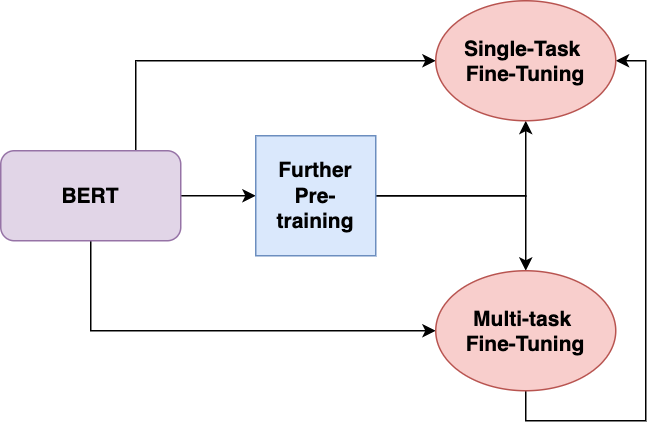
\includegraphics[width=0.8\textwidth]{fig4_paths.png}
  \caption{要改进你的 BERT 模型，有几条不同的路径可以选择，包括：(1) 在 BERT 的原始目标上做额外预训练，(2) 直接在单个任务上微调你的模型，(3) 对你的 BERT 模型进行多任务训练。}
  \label{fig:paths}
\end{figure}

\subsubsection{额外预训练（Additional Pretraining）}

\textbf{原论文：}《How to Fine-Tune BERT for Text Classification?》~\cite{sun2019how}

如第 3 节所述，BERT 是在通用领域训练的，其数据分布与我们将用于给你评分的那些数据集不同。改进你模型的一个自然方法是，用目标领域的数据进一步预训练你的 BERT 模型。这将涉及用我们提供的训练数据集，实现并训练第 3 节所述的掩码语言模型目标或 token 预测。有关 BERT 预训练的更多细节，参见文献~\cite{devlin2018bert}。

\subsubsection{多重负样本排序损失学习（Multiple Negatives Ranking Loss Learning）}

\textbf{原论文：}《Efficient Natural Language Response Suggestion for Smart Reply》~\cite{henderson2017efficient}

改进嵌入的另一个有效方法是，用多重负样本排序损失（Multiple Negative Ranking Loss）\footnote{\url{https://www.sbert.net/docs/package_reference/losses.html}} 来微调你的模型。使用该损失函数时，训练数据由一组 $K$ 个句子对 $[(a_1, b_1), \dots, (a_n, b_n)]$ 组成，其中 $a_i, b_i$ 被标注为相似句子，而所有 $i \neq j$ 的 $(a_i, b_j)$ 都不是相似句子。然后，损失函数在最小化 $a_i, b_i$ 之间距离的同时，最大化 $i \neq j$ 的 $(a_i, b_j)$ 之间的距离。具体来说，训练就是最小化数据的近似平均负对数概率。对于单个 batch，其计算方式为：

\begin{equation*}
\begin{aligned}
J(x, y, \theta) &= -\frac{1}{K}\sum_{i=1}^{K} \log P_{approx}(y_i \mid x_i) \\
                &= -\frac{1}{K}\sum_{i=1}^{K}\left( S(x_i, y_i) - \log\sum_{j=1}^{K} e^{S(x_i, y_j)} \right),
\end{aligned}
\end{equation*}

其中 $\theta$ 表示用于计算 $S$（一个评分函数）的词嵌入和神经网络参数。更多细节参见 sbert.net\footnote{\url{https://www.sbert.net/examples/training/nli/README.html\#multiplenegativesrankingloss}} 和 Henderson 等人~\cite{henderson2017efficient}。

\subsubsection{余弦相似度微调（Cosine-Similarity Fine-Tuning）}

\textbf{原论文：}《Sentence-BERT: Sentence Embeddings using Siamese BERT-Networks》~\cite{reimers2019sentence}

进一步的微调可以继续提升你的 BERT 模型在某个预选任务上的表现。两个嵌入之间的相似度通常用它们的余弦相似度来计算。因此，改进嵌入的一个可能方法，是在 SemEval 数据集上微调时使用 \texttt{CosineEmbeddingLoss}\footnote{\url{https://pytorch.org/docs/stable/generated/torch.nn.CosineEmbeddingLoss.html}}。在这种设定下，含义等价的句子余弦相似度为 1，不相关的句子余弦相似度为 0。

\subsubsection{带正则化优化的微调（Fine-Tuning with Regularized Optimization）}

\textbf{原论文：}《SMART: Robust and Efficient Fine-Tuning for Pre-trained Natural Language Models through Principled Regularized Optimization》~\cite{jiang2019smart}

激进的微调常常会导致过拟合，从而可能使模型无法泛化到未见过的数据。为了以有原则的方式对抗这一点，Jiang 等人提出：(1) \textbf{平滑诱导正则化}（smoothness-inducing regularization），它能有效管理模型的复杂度；以及 (2) \textbf{Bregman 近端点优化}，它是信赖域方法的一种实例，可以防止激进的更新。

\textbf{平滑诱导对抗正则化} 具体来说，给定模型 $f(\cdot; \theta)$ 以及目标任务的 $n$ 个数据点 $\{(x_i, y_i)\}_{i=1}^{n}$，其中 $x_i$ 表示从语言模型第一个嵌入层得到的输入句子嵌入，$y_i$ 是相关标签，Jiang 等人的方法本质上求解以下微调优化问题：

\begin{equation}
\min_{\theta} \; L(\theta) + \lambda_s R_s(\theta)
\end{equation}

其中 $L(\theta)$ 是损失函数，定义为：

\begin{equation}
L(\theta) = \frac{1}{n}\sum_{i=1}^{n} l(f(x_i; \theta), y_i),
\end{equation}

$l(\cdot, \cdot)$ 是取决于目标任务的损失函数，$\lambda_s > 0$ 是调优参数，$R_s(\theta)$ 是平滑诱导正则项，定义为：

\begin{equation}
R_s(\theta) = \frac{1}{n}\sum_{i=1}^{n} \max_{\lVert \tilde{x}_i - x_i \rVert_p \le \epsilon} l_s(f(\tilde{x}_i; \theta), f(x_i; \theta)),
\end{equation}

其中 $\epsilon > 0$ 是调优参数。注意，对于分类任务，$f(\cdot; \theta)$ 输出一个概率单纯形，$l_s$ 取对称 KL 散度，即：

\begin{equation}
l_s(P, Q) = D_{KL}(P \Vert Q) + D_{KL}(Q \Vert P)
\end{equation}

\textbf{Bregman 近端点优化} Jiang 等人还提出了一类 Bregman 近端点优化方法\footnote{\url{https://www.stat.cmu.edu/~ryantibs/convexopt/lectures/bregman.pdf}}，用于求解公式 (7)。这类优化方法在每次迭代都施加一个强惩罚，以防止模型激进更新。具体来说，它们用预训练模型作为初始化，记为 $f(\cdot; \theta_0)$。在第 $(t+1)$ 次迭代，原始 Bregman 近端点（VBPP）方法取：

\begin{equation}
\theta_{t+1} = \arg\min_{\theta} \; F(\theta) + \mu D_{Breg}(\theta, \theta_t)
\end{equation}

其中 $\mu > 0$ 是调优参数，$D_{Breg}(\cdot, \cdot)$ 是 Bregman 散度，定义为：

\begin{equation}
D_{Breg}(\theta, \theta_t) = l_s(f(\tilde{x}_i; \theta), f(x_i; \theta_t))
\end{equation}

更多细节参见 \url{https://github.com/namisan/mt-dnn} 和文献~\cite{jiang2019smart}。

\subsubsection{多任务微调（Multitask Fine-Tuning）}

\textbf{原论文：}《BERT and PALs: Projected Attention Layers for Efficient Adaptation in Multi-Task Learning》~\cite{stickland2019bert}；《MTRec: Multi-Task Learning over BERT for News Recommendation》~\cite{bi2022mtrec}；《Gradient surgery for multi-task learning》~\cite{yu2020gradient}

与其在单个任务上微调 BERT，你也可以改用多任务学习来更新 BERT。例如，Bi 等人~\cite{bi2022mtrec} 使用多任务学习，把类别分类任务和命名实体识别任务的损失加在一起：

\begin{equation}
L_{total} = L_{task1} + L_{task2}
\end{equation}

然而，使用多任务学习并不总是有益的，这取决于模型如何微调。不同任务的梯度方向可能会相互冲突。Yu 等人~\cite{yu2020gradient} 推荐了一种称为\textbf{Gradient Surgery}（梯度外科手术）的技术，它把第 $i$ 个任务的梯度 $g_i$ 投影到另一个冲突任务梯度 $g_j$ 的法平面上：

\begin{equation}
g_i = g_i - \frac{g_i \cdot g_j}{\lVert g_j \rVert^2} \cdot g_j
\end{equation}

\subsubsection{对比学习（Contrastive Learning）}

\textbf{原论文：}《Simple Contrastive Learning of Sentence Embeddings》~\cite{gao2021simcse}

Gao 等人~\cite{gao2021simcse} 提出了一个简单的对比学习框架，名为 SimCSE，它既能用于无标签数据也能用于有标签数据。无监督 SimCSE 简单地取一个输入句子，在对比学习框架中预测它自己，只用标准 dropout 作为噪声。相比之下，有监督 SimCSE 把 NLI 数据集中的标注句子对纳入对比学习，用蕴含对（entailment pairs）作为正样本，用矛盾对（contradiction pairs）作为难负样本。你可以利用类似的方法，在你不同的模型上改进句子嵌入。

\subsubsection{参数高效微调方法（Parameter Efficient Finetuning Methods）}

\textbf{原论文：}《LoRA: Low-Rank Adaptation of Large Language Models》~\cite{hu2022lora}；《DoRA: Weight-Decomposed Low-Rank Adaptation》~\cite{liu2024dora}

存在若干技术可以在保持性能的同时，减少微调语言模型所需的内存/运行时间。其中一种技术是 LoRA~\cite{hu2022lora}，其动机是一个假设：即使在完全微调中，对语言模型权重矩阵的更新本质上也是低秩的。因此，给定一个预训练模型，Hu 等人~\cite{hu2022lora} 提出把模型的权重矩阵 $W$ 重新参数化为 $W_0 + BA$，其中 $W_0$ 表示预训练得到的权重矩阵，$A, B$ 是微调时新增的参数。这里，如果 $W_0$ 的形状是 $d \times k$，那么 $B$ 和 $A$ 的形状将分别是 $d \times r$ 和 $r \times k$，其中 $r \ll d, k$。该技术的一个显著优势是，优化器所需的内存更少（优化器需要为每个被优化的参数存储一些状态）。

LoRA 有可能比标准微调表现更差。Liu 等人~\cite{liu2024dora} 提出 DoRA，旨在解决造成这种情况的原因。在 DoRA 中，预训练的 $d \times k$ 权重矩阵 $W_0$ 现在被重新参数化为 $m \cdot \frac{V}{\lVert V \rVert_c}$，其中 $V$ 是一个 $d \times k$ 矩阵，$\lVert V \rVert_c$ 是一个 $1 \times k$ 向量，其第 $i$ 个元素是 $V$ 第 $i$ 列的模长，$m$ 是一个 $1 \times k$ 向量，包含每一列一个可学习的模长。换句话说，DoRA 试图把对 $W_0$ 模长的更新与对 $W_0$ 方向的更新解耦开来。

之后，方向分量 $V$ 用 LoRA 更新。换句话说，$V$ 本身被重新参数化为 $W_0 + BA$，其中 $B$ 和 $A$ 的形状分别是 $d \times r$ 和 $r \times k$，其中 $r \ll d, k$。之后，只有 $B$ 和 $A$ 会接收更新。为了显著减少反向传播所需的内存，Liu 等人提出把因子 $\frac{1}{\lVert V \rVert_c}$ 当作常数，并把它从反向传播图中分离出来（同时其余部分照常计算）。

\subsubsection{额外数据集（Additional Datasets）}

\textbf{原论文：}《SMART: Robust and Efficient Fine-Tuning for Pre-trained Natural Language Models through Principled Regularized Optimization》~\cite{jiang2019smart}；《Sentence-BERT: Sentence Embeddings using Siamese BERT-Networks》~\cite{reimers2019sentence}

在不同数据集上微调 BERT 模型是你可以采用的另一种方法。有大量不同的数据集和任务可以潜在地应用到你的模型上，以获得更丰富、更鲁棒的嵌入。以下是一些示例数据集：

\begin{itemize}[leftmargin=1.5em]
  \item \url{https://arxiv.org/abs/1508.05326}
  \item \url{http://sbert.net/datasets/paraphrases}
  \item \url{https://arxiv.org/abs/1704.05426}
\end{itemize}

\subsubsection{额外的输入特征（Additional input features）}

尽管深度学习能够端到端地学习而不需要特征工程，但事实证明，使用正确的输入特征（例如词性标签、命名实体类型等）仍然可以显著提升性能。如果你实现了这样的模型，请在报告中评论特征工程与端到端学习之间的权衡。

\subsubsection{其他改进（Other improvements）}

还有许多其他微妙的改进性能的方法。本节中的建议只是一些例子；运行必要的实验并做出必要的比较需要时间。

\begin{itemize}[leftmargin=1.5em]
  \item \textbf{正则化。}基线代码使用了 dropout。你可以进一步试验不同的 dropout 值和不同类型的正则化。
  \item \textbf{共享权重。}基线代码勾勒了一种方式，用不同的头来预测句子是否为释义、它们的语义相似度以及每个句子的情感。你也许可以在任务头之间共享一些层，以提升性能。
  \item \textbf{模型大小与层数。}对于任何模型，你都可以尝试增大层的大小或增加层的数量。
  \item \textbf{优化算法。}基线使用 Adam 优化器。PyTorch 支持许多其他优化算法。你也可以尝试改变学习率。
  \item \textbf{集成。}集成几乎总能提升性能，所以试着把你几个模型组合起来做最终提交。不过，集成的计算开销更大。
  \item \textbf{超参数优化。}虽然我们为各种超参数提供了一些默认值，但这些默认值不一定能带来最好的结果。另一种方法是进行超参数搜索，为你的模型找到最佳超参数。
\end{itemize}

\subsubsection{其他方法（Other Approaches）}

我们在这里展示的模型和技术远非穷尽。有许多已发表的论文涉及相关或不相关的任务\footnote{\url{http://nlpprogress.com/}}。这些论文可能包含一些有趣的思路，你可以应用它们来构建更鲁棒、语义更丰富的嵌入。

\subsection{提交说明}

你将在 Gradescope 上提交本项目的扩展部分。

\begin{enumerate}
  \item 运行 \texttt{prepare\_submit.py}。该命令应把你所有的 \texttt{*.py} 文件和预测 \texttt{*.csv} 文件打包进一个 zip 文件。
  \item 验证生成的 \texttt{cs224n\_default\_final\_project\_submission.zip} 文件包含：你在三个下游任务上的模型预测（位于 \texttt{predictions/*} 目录），以及复现你结果所需的全部代码。
  \item 将你的 \texttt{cs224n\_default\_final\_project\_submission.zip} 文件上传到 Gradescope 上相应的作业。
\end{enumerate}

%=====================================================================
\section{提交到排行榜（Submitting to the Leaderboard）}

\subsection{概述（Overview）}

除了提交你的 \texttt{.zip} 文件外，你还应该把你对三个数据集的预测提交到两个 Gradescope 排行榜\footnote{我们会在排行榜上展示你最终模型在 SST 测试/开发数据集上的准确率、在 Quora 测试/开发数据集上的准确率、在 STS SemEval 测试/开发数据集上的 Pearson 分数，以及跨全部三个任务的综合分数。}。

你可以在开发排行榜上任意次提交，但在测试排行榜上只允许 3 次成功提交。对于你的最终报告，我们会要求你选择一个单一的测试排行榜提交，作为你最终成绩的考量。因此，你必须在测试排行榜上至少提交一次，但要小心，不要在你完成最佳模型开发之前就用完你的测试提交次数。

向排行榜提交与在 Gradescope 上提交任何其他作业类似，只不过你的提交是一个对开发/测试集的预测 CSV 文件。在高层面，SST 数据集的提交文件应大致如下：

\begin{lstlisting}[numbers=none]
id, Predicted_Sentiment
001fefa37a13cdd53fd82f617, 4
00415cf9abb539fbb7989beba, 2
00a4cc38bd041e9a4c4e545ff, 1
...
fffcaebf1e674a54ecb3c39df, 3
\end{lstlisting}

STS 数据集的提交文件应大致如下：

\begin{lstlisting}[numbers=none]
id, Predicted_Similarity
8f4d49b9f4558f9e45423e84c, 1.000
1c5cd37407630a3ba19a0f2ad, 0.4051
318c885e36cc9e6f6bb7de7dd, 0.2138
...
4e1ef3b635d01039a8a8f059b, 0.7462
\end{lstlisting}

释义数据集的提交文件应大致如下：

\begin{lstlisting}[numbers=none]
id, Predicted_Is_Paraphrase
872887985e1e0f2dd5b690ffd, 1
472398907a6adb9ed2f660550, 0
c3ceaaed421cc008282efdf8a, 0
...
5e10dfc4ac8ae205f3e114445, 1
\end{lstlisting}

表头是必需的，同时第一列必须是每个样本的 25 位十六进制 ID（ID 在各测试/开发文件中定义），最后一列是你预测的答案（没有答案则为空字符串）。行可以按任意顺序排列。你必须为每个样本都提交一个预测。

\subsection{提交步骤（Submission Steps）}

以下是向排行榜提交的具体步骤：

\begin{enumerate}
  \item 用你的 multitask BERT 模型生成预测 \texttt{.csv} 文件。
  \item 为你的划分（DEV 或 TEST）选择正确的排行榜。
  \item 上传你的提交并等待分数。提交输出会告诉你该提交在开发/测试数据集上的准确率/Pearson 相关系数。它还会显示你当前表现与你最佳提交之间的差值。你在排行榜上的排名取决于你的最佳提交，而不一定是你最近的提交。
\end{enumerate}

如果出现任何问题，应该有有用的错误信息。如果你遇到看不懂的错误，请在 Ed 上发帖提问。

%=====================================================================
\section{评分标准（Grading Criteria）}

最终项目将进行整体性（holistic）评分。这意味着我们在确定你的分数时会考量许多因素：你方法的\textbf{创造性}、\textbf{复杂度}和\textbf{技术正确性}，你探索和比较各种方法的\textbf{彻底程度}，你\textbf{结果的强度}，你所投入的\textbf{努力}，以及你\textbf{报告、评测和误差分析的质量}。一般来说，实现更复杂的模型代表更多的努力，实现更不寻常的模型（例如本讲义中未提到的模型）代表更多的创造性。你并不被要求追求原创想法，但本课程中最优秀的项目会超越本讲义所述的想法，实际上甚至可能成为已发表的工作！

与往年一样，对于本项目的第二部分，你成绩的一个方面是你相对于整个排行榜的表现。注意，你在排行榜上结果的强度只是我们评分时考虑的众多因素之一。我们的重点在于评估你\textbf{推理充分的研究问题、解释和实验}，这些需要清晰地评估那些问题。

不存在预定义的准确率（SST、Quora）或 Pearson 分数（SemEval）来保证好成绩。同样，也不存在预定义的规则，规定第 5 节（或其他地方）中哪些扩展能保证好成绩。实现少量但结果良好、实验/分析彻底的东西，比实现大量不起作用或勉强起作用的东西更好。此外，你报告和实验的质量也很重要：我们期望你能令人信服地证明你的技术是有效的，并描述它们为什么有效（或者对不奏效的情况清楚地阐明推理）。

与所有最终项目一样，更大的团队被期望做相应更大的项目。我们期望人数更多的团队实现更复杂的东西、进行更彻底的实验、取得更好的结果。

%=====================================================================
\section{荣誉准则（Honor Code）}

任何适用于自定义最终项目的荣誉准则，一般也适用于默认最终项目。以下是一些与默认最终项目特别相关的准则：

\begin{enumerate}
  \item 你不可以使用既有的 minBERT 实现。
  \item 你不允许在你的系统中使用预训练的上下文嵌入（如 ELMO、GPT 等）。你可以使用其他既有的 NLP 工具，如词性标注器、依存句法分析器和共指消解模块，只要它们不是建立在预训练上下文嵌入之上的。
  \item 你可以自由地与其他团队讨论想法和实现细节（实际上，我们鼓励这样做！）。但是，在任何情况下，你都不能查看另一个 CS 224N 团队的代码，或将他们的代码纳入你的项目。
  \item 如别处所述，以任何方式使用官方 SST、Quora 或 SemEval 数据集，都构成荣誉准则违规。
  \item 在课程结束之前，不要公开分享你的代码（例如放在公开的 GitHub 仓库中）。
\end{enumerate}

%=====================================================================
\begin{thebibliography}{19}
\small

\bibitem{devlin2018bert} Jacob Devlin, Ming-Wei Chang, Kenton Lee, and Kristina Toutanova. Bert: Pre-training of deep bidirectional transformers for language understanding. \textit{arXiv preprint arXiv:1810.04805}, 2018.

\bibitem{socher2013recursive} Richard Socher, Alex Perelygin, Jean Wu, Jason Chuang, Christopher D Manning, Andrew Y Ng, and Christopher Potts. Recursive deep models for semantic compositionality over a sentiment treebank. In \textit{Proceedings of the 2013 conference on empirical methods in natural language processing}, pages 1631--1642, 2013.

\bibitem{fernando2008semantic} Samuel Fernando and Mark Stevenson. A semantic similarity approach to paraphrase detection. In \textit{Proceedings of the 11th annual research colloquium of the UK special interest group for computational linguistics}, pages 45--52, 2008.

\bibitem{agirre2013sem} Eneko Agirre, Daniel Cer, Mona Diab, Aitor Gonzalez-Agirre, and Weiwei Guo. *SEM 2013 shared task: Semantic textual similarity. In \textit{Second joint conference on lexical and computational semantics (*SEM), volume 1: proceedings of the Main conference and the shared task: semantic textual similarity}, pages 32--43, 2013.

\bibitem{vaswani2017attention} Ashish Vaswani, Noam Shazeer, Niki Parmar, Jakob Uszkoreit, Llion Jones, Aidan N Gomez, Łukasz Kaiser, and Illia Polosukhin. Attention is all you need. In \textit{Advances in Neural Information Processing Systems}, pages 5998--6008, 2017.

\bibitem{ba2016layer} Jimmy Lei Ba, Jamie Ryan Kiros, and Geoffrey E Hinton. Layer normalization. \textit{arXiv preprint arXiv:1607.06450}, 2016.

\bibitem{hendrycks2016gaussian} Dan Hendrycks and Kevin Gimpel. Gaussian error linear units (gelus). \textit{arXiv preprint arXiv:1606.08415}, 2016.

\bibitem{loshchilov2017decoupled} Ilya Loshchilov and Frank Hutter. Decoupled weight decay regularization. \textit{arXiv preprint arXiv:1711.05101}, 2017.

\bibitem{kingma2014adam} Diederik P Kingma and Jimmy Ba. Adam: A method for stochastic optimization. \textit{arXiv preprint arXiv:1412.6980}, 2014.

\bibitem{sun2019how} Chi Sun, Xipeng Qiu, Yige Xu, and Xuanjing Huang. How to fine-tune bert for text classification? In \textit{Chinese Computational Linguistics: 18th China National Conference, CCL 2019, Kunming, China, October 18--20, 2019, Proceedings 18}, pages 194--206. Springer, 2019.

\bibitem{henderson2017efficient} Matthew Henderson, Rami Al-Rfou, Brian Strope, Yun-Hsuan Sung, László Lukács, Ruiqi Guo, Sanjiv Kumar, Balint Miklos, and Ray Kurzweil. Efficient natural language response suggestion for smart reply. \textit{arXiv preprint arXiv:1705.00652}, 2017.

\bibitem{reimers2019sentence} Nils Reimers and Iryna Gurevych. Sentence-bert: Sentence embeddings using siamese bert-networks. In \textit{Proceedings of the 2019 Conference on Empirical Methods in Natural Language Processing and the 9th International Joint Conference on Natural Language Processing (EMNLP-IJCNLP)}, pages 3982--3992, 2019.

\bibitem{jiang2019smart} Haoming Jiang, Pengcheng He, Weizhu Chen, Xiaodong Liu, Jianfeng Gao, and Tuo Zhao. Smart: Robust and efficient fine-tuning for pre-trained natural language models through principled regularized optimization. \textit{arXiv preprint arXiv:1911.03437}, 2019.

\bibitem{stickland2019bert} Asa Cooper Stickland and Iain Murray. Bert and pals: Projected attention layers for efficient adaptation in multi-task learning. In \textit{International Conference on Machine Learning}, pages 5986--5995. PMLR, 2019.

\bibitem{bi2022mtrec} Qiwei Bi, Jian Li, Lifeng Shang, Xin Jiang, Qun Liu, and Hanfang Yang. Mtrec: Multi-task learning over bert for news recommendation. In \textit{Findings of the Association for Computational Linguistics: ACL 2022}, pages 2663--2669, 2022.

\bibitem{yu2020gradient} Tianhe Yu, Saurabh Kumar, Abhishek Gupta, Sergey Levine, Karol Hausman, and Chelsea Finn. Gradient surgery for multi-task learning. \textit{Advances in Neural Information Processing Systems}, 33:5824--5836, 2020.

\bibitem{gao2021simcse} Tianyu Gao, Xingcheng Yao, and Danqi Chen. SimCSE: Simple contrastive learning of sentence embeddings. In \textit{Empirical Methods in Natural Language Processing (EMNLP)}, 2021.

\bibitem{hu2022lora} Edward J. Hu, Yelong Shen, Phillip Wallis, Zeyuan Allen-Zhu, Yuanzhi Li, Shean Wang, Lu Wang, and Weizhu Chen. Lora: Low-rank adaptation of large language models. In \textit{The Tenth International Conference on Learning Representations, ICLR 2022, Virtual Event, April 25-29, 2022}. OpenReview.net, 2022.

\bibitem{liu2024dora} Shih-Yang Liu, Chien-Yi Wang, Hongxu Yin, Pavlo Molchanov, Yu-Chiang Frank Wang, Kwang-Ting Cheng, and Min-Hung Chen. Dora: Weight-decomposed low-rank adaptation. \textit{CoRR}, abs/2402.09353, 2024.

\end{thebibliography}

\end{document}
